\chapter{Lossy Passive Relays}
\label{sec:lossyrel}

In this chapter, the effect of lossy passive relays will be explored.
In the beginning we justified the choice of considering only pure imaginary impedances at the relays, by the fact, that this results in loss less relays.
In the following we will allow the impedances to become complex, with a strict positive real part, i.e.
$\mat{Z}_\text{Rel} = \mat{R}_\text{Rel} + j\mat{X}_\text{Rel}$ with $R_\text{Rel}[i]>=0,\forall i\in[1,\cdots,N_{Rel}]$.

It is obvious, that the performance of this system must be strictly larger than allowing only loss less relays, as we can set the real part to zero and therefore we would get the same result.

\begin{figure}[h]
\centering
  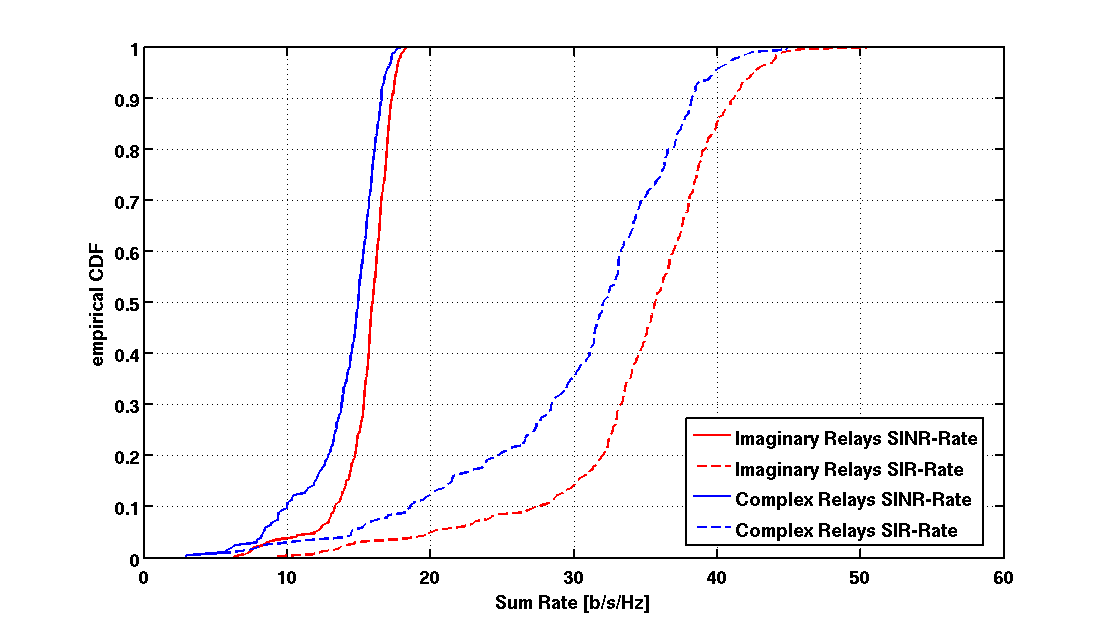
\includegraphics[width=\linewidth]{images/Imagvscomp.png}
\caption{Comparison of loss less and lossy relays.}
\label{fig:lossyrel}
\end{figure}

Figure~\ref{fig:lossyrel} shows the performance of the loss less relays in red, as we know them from the previous chapters.
In blue the performance of the lossy relays is given.
We see, that the performance is lower than the performance of the loss less relays, which is contradicting to the statement above.
This leads to the conclusion, that the performance of the solver is worse, when the degree of freedom is larger.
Approaches to prevent the solver in running into these lower rates would be a pre-optimization of the loss less relays and afterwards performing an optimization with lossy relays using the results from the red curve as initial values.



\chapter{Nossek}
\label{sec:nossek}


Description according to Nossek's way~\cite{Nossek}:

Describing the relays by the Matching Network

\begin{align}
\label{eq:nossek_matching}
\mat{Z}_\text{M11}[\text{M}+\left(1:N_\text{Rel}\right)] &= \text{diag}\left(\vec{s}\right)\\
\mat{Z}_\text{M12}[\text{M}+\left(1:N_\text{Rel}\right)] &= 
	\mat{Z}_\text{M21}[\text{M}+\left(1:N_\text{Rel}\right)] = \mat{0}\\
\mat{Z}_\text{M22}[\text{M}+\left(1:N_\text{Rel}\right)] &= \text{undef.}\\
\mat{Z}_\text{M11} &=
\begin{bmatrix}
\text{M}_\text{1,11} & \cdots & 0 &\\
 \vdots & \ddots & \vdots & \mat{0} \\
 0 & \cdots & \text{M}_\text{M,11}&\\
 & \mat{0}& & \text{diag}\left(\mat{s}\right)
\end{bmatrix}\\
\mat{Z}_\text{M12}&=
\begin{bmatrix}
\text{M}_\text{1,12} & \cdots& 0&\\
\vdots & \ddots & \vdots & \mat{0}\\
0 & \cdots & \text{M}_\text{M,12}&\\
& \mat{0} &	& 0\cdot\mat{I}_{N_\text{Relays}}
\end{bmatrix}
\end{align}

this leads to the input impedance
\begin{align}
\label{eq:nossek_matching}
\mat{Z}_\text{inM}[\text{M}+\left(1:N_\text{Rel}\right)] &= \text{diag}\left(\mat{s}\right)
\end{align}



The transfer matrix
\begin{align}
\label{eq:nossek_transf}
\mat{H}_\text{L,0} &= \frac{z_l d}{z_l + g}\mat{D}\mat{F}_R,\quad\text{with}\\
\mat{D} &= \left(c\mat{I} + \mat{Z}_R\right)^{-1},\\
\mat{F}_R &= \mat{Z}_\text{M12}\left(\mat{Z}_\text{M11}+\mat{Z}_\text{C}\right)^{-1},\quad\text{and}\\
\mat{Z}_R &= \mat{Z}_\text{M22} + \mat{F}_R\mat{Z}_\text{M12}
\end{align}

\begin{align}
\vec{v}_\text{L} &= \mat{H}_\text{L,0}\cdot\vec{v}_o + \vec{n}\\
\vec{v}_\text{L} &= \mat{H}_\text{L,0}\cdot\mat{H}_{j}^{\text{sp}}\cdot\vec{v}_j
\end{align}



MU-MIMO TF

\begin{align}
\label{eq:nossek_transf}
\vec{y}_i &= \mat{A}_{i,i}\vec{x}_i + 
	\sum_{j=0,j\neq i}^{N_\text{User}-1} \mat{A}_{i,j}\vec{x}_j + \vec{n}\\
\mat{A} &= \mat{H}_\text{L,0}\cdot\mat{H}^{\text{sp}}
\end{align}

User 0 achievable rate:
\begin{align}
\label{eq:achiev_rate}
r_i &= \text{log}_2\left(\text{det}\left(\mat{K}_{\text{s},i}\left(\mat{K}_{\text{i},i}+\mat{K}_{\text{n},i}\right)^{-1}+\mat{I}_{N_R}\right)\right)\\
 &=\text{log}_2\left(
	\text{det}\left(\mat{K}_{\text{s},i}+
		\mat{K}_{\text{i},i}+\mat{K}_{\text{n},i}\right)\right) -
	\text{log}_2\left(\text{det}\left(\mat{K}_{\text{i},i}+\mat{K}_{\text{n},i}\right)\right).
\end{align}

Signal Cov
\begin{align}
\mat{K}_{\text{s},i}=\mathbb{E}[\vec{v}_\text{L}^\text{s}\vec{v}_\text{L}^{\text{s}^H}] &= 
	\mat{H}_\text{L,0} \cdot \mat{H}_{i}^{\text{sp}} \cdot 
	\mathbb{E}[\vec{v}_{i}\vec{v}_{i}^H] \cdot 
	\mat{H}_{i}^{\text{sp}^H} \cdot \mat{H}_\text{L,0}^H,\\
\mat{K}_{\text{s},i}=\mathbb{E}[\vec{v}_\text{L}^\text{s}\vec{v}_\text{L}^{\text{s}^H}] &= 
	\mat{H}_\text{L,0} \cdot \mat{H}_{i}^{\text{sp}} \cdot  
	\mat{H}_{i}^{\text{sp}^H} \cdot \mat{H}_\text{L,0}^H\cdot P_i
\end{align}
Interference Cov
\begin{align}
\mat{K}_{\text{i},i}=\mathbb{E}[\vec{v}_\text{L}^\text{i}\vec{v}_\text{L}^{\text{i}^H}] &= \sum_{j=0,j\neq i}^{N_\text{User}-1} 
	\mat{H}_\text{L,0} \cdot \mat{H}_{j}^{\text{sp}} \cdot 
	\mathbb{E}[\vec{v}_{j}\vec{v}_{j}^H] \cdot 
	\mat{H}_{j}^{\text{sp}^H} \cdot \mat{H}_\text{L,0}^H,\\
	&= \mat{H}_\text{L,0} \left(\sum_{j=1}^{N_\text{User}-1} 
	\cdot \mat{H}_{j}^{\text{sp}} \cdot 
	\mathbb{E}[\vec{v}_{j}\vec{v}_{j}^H] \cdot 
	\mat{H}_{j}^{\text{sp}^H}\right) \cdot \mat{H}_\text{L,0}^H,\\
\mat{K}_{\text{i},i}=\mathbb{E}[\vec{v}_\text{L}^\text{i}\vec{v}_\text{L}^{\text{i}^H}] &= \sum_{j=0,j\neq i}^{N_\text{User}-1} 
	\mat{H}_\text{L,0} \cdot \mat{H}_{j}^{\text{sp}} \cdot 
	\mat{H}_{j}^{\text{sp}^H} \cdot \mat{H}_\text{L,0}^H\cdot P_j,\\
	&= \mat{H}_\text{L,0} \left(\sum_{j=1}^{N_\text{User}-1} 
	\cdot \mat{H}_{j}^{\text{sp}} \cdot
	\mat{H}_{j}^{\text{sp}^H}\right) \cdot \mat{H}_\text{L,0}^H\cdot P_j
\end{align}

